\chapter{Exploration}
This chapter describes the process of the index concepts in Apache Solr, explains how the apache solr works when indexing  points out some of the improvements that should be made. It also takes a deeper look in the Facet Api \footnote{\url{http://www.drupal.org/project/facetapi}}module to see how it is structured and where it could use improvements. 
Finally Apache Solr was benchmarked with different configurations to find out the most optimal ones.

\section{Apache Solr}
\paragraph{Version conflicts}
Apache Solr exists out of a couple parts. The analysis part tries to explain you all it entails. When Drupal 6 came out and became popular, there was only one version of Apache Solr available. This was version 1.4 and was not yet merged with the Lucene branch. Solr's version number was synced with Lucene following the Lucene/Solr merge, so Solr 3.1 contains Lucene 3.1. Solr 3.1 is the first release after Solr 1.4.1. All the explanation that follows will be for Solr 3.x since this is the version that is used and was aimed at during the creation of this project.

\paragraph{Fields}
There are different field types defined in the original schema.xml that used to come with the module. A field type has four types of information.
\begin{itemize}
  \item The name of the field type
  \item An implementation class name
  \item If the field type is TextField, a description of the field analysis for the field type
  \item Field attributes
\end{itemize}
To illustrate this there is listing \ref{code:fieldtypedefinition} as an example of a field type definition as it is used in the schema provided with the Apache Solr Module and also a list of all possible field types in listing \ref{lst:fieldtypedefinition}

\begin{longtable}{| p{4cm} | p{11cm} |}
    \hline
    Class & Description \\ \hline
    BCDIntField & Binary-coded decimal (BCD) integer. BCD is a relatively inefficient 
    encoding that offers the benefits of quick decimal calculations and quick conversion to a string. \\ \hline
    BCDLongField & BCD long integer \\ \hline
    BCDStrField & BCD string \\ \hline
    *BinaryField & Binary data \\ \hline
    *BoolField & Contains either true or false. Values of "1", "t", or "T" in the first character are interpreted as true. Any other values in the first character are interpreted as false. \\ \hline
    ByteField & Contains an array of bytes. \\ \hline
    *DateField & Represents a point in time with millisecond precision. \\ \hline
    DoubleField & Double (64-bit IEEE floating point) \\ \hline
    ExternalFileField & Pulls values from a file on disk. \\ \hline
    FloatField & Floating point (32-bit IEEE floating point) \\ \hline
    IntField & Integer (32-bit signed integer) \\ \hline
    LongField & Long integer (64-bit signed integer) \\ \hline
    *RandomSortField & Does not contain a value. Queries that sort on this field type will return results in random order. Use a dynamic field to use this feature. \\ \hline
    ShortField & Short integer \\ \hline
    SortableDoubleField & The Sortable* fields provide correct numeric sorting. If you use the plain types (DoubleField, IntField, and so on) sorting will be lexicographical instead of numeric. \\ \hline
    SortableFloatField & Numerically sorted floating point \\ \hline
    SortableIntField & Numerically sorted integer \\ \hline
    SortableLongField & Numerically sorted long integer \\ \hline
    *StrField & String (UTF-8 encoded string or Unicode) \\ \hline
    *TextField & Text, usually multiple words or tokens \\ \hline
    *TrieDateField & Date field accessible for Lucene TrieRange processing \\ \hline
    *TrieDoubleField & Double field accessible Lucene TrieRange processing \\ \hline
    TrieField & If this type is used, a "type" attribute must also be specified, with a value of either: integer, long, float, double, date. Using this field is the same as using any of the Trie*Fields. \\ \hline
    *TrieFloatField & Floating point field accessible Lucene TrieRange processing \\ \hline
    *TrieIntField & Int field accessible Lucene TrieRange processing \\ \hline
    *TrieLongField & Long field accessible Lucene TrieRange processing \\ \hline
    *PointType & For spatial search: An arbitrary n-dimensional point, useful for searching sources such as blueprints or CAD drawings. \\ \hline
    *LatLonType &  Latitude/Longitude as a 2 dimensional point. Latitude is always specified first.\\ \hline
    *GeoHashField & Representing a Geohash\footnote{Geohash is a defined standard. More on wikipedia : \url{http://en.wikipedia.org/wiki/Geohash}} field. The field is provided as a lat/lon pair and is internally represented as a string.\\ \hline
    UUIDField & Universally Unique Identifier (UUID). Pass in a value of "NEW" and Solr will create a new UUID. \\ 
     \hline
\end{longtable}
\captionof{listing}{All field type definitions. Marked with a star are the ones that are used in the Apache Solr Search Integration module for Drupal  \label{lst:fieldtypedefinition}}

\paragraph{Field properties}
Important to know is that each of these fields that is shown in listing \ref{lst:fieldtypedefinition} have configurable values. Drupal uses these properties to map different dynamic fields to specific types with specific configurations. 
These dynamic fields are what we call fields from the Field API (Drupal 7) or from the Content Construction Kit (CCK, Drupal 6). With these modules it is possible to add different fields to content types\footnote{Content types are a way of defining structured data that will be inputted by users}

\begin{longtable}{| p{4.5cm} | p{8.5cm} | p{2cm} |}
    \hline
    Field Property & Description & Values \\ \hline
    indexed & If true, the value of the field can be used in queries to retrieve matching documents & true or false\\ \hline
    stored &  If true, the actual value of the field can be retrieved by queries & true or false\\ \hline
    sortMissingFirst / sortMissingLast & Control the placement of documents when a sort field is not present. As of Solr 3.5, these work for all numeric fields, including Trie and date fields. & true or false\\ \hline
    multiValued & If true, indicates that a single document might contain multiple values for this field type & true or false\\ \hline
    positionIncrementGap & For multivalued fields, specifies a distance between multiple values, which prevents spurious phrase matches & integer\\ \hline
    omitNorms & If true, omits the norms associated with this field (this disables length normalization and index-time boosting for the field, and saves some memory). Only full-text fields or fields that need an index-time boost need norms. & true or false\\ \hline
    omitTermFreqAndPositions & If true, omits term frequency, positions, and payloads from postings for this field. This can be a performance boost for fields that don't require that information. It also reduces the storage space required for the index. Queries that rely on position that are issued on a field with this option will silently fail to find documents. This property defaults to true for all fields that are not text fields. & true or false\\ \hline
    autoGeneratePhraseQueries & For text fields. If true, Solr automatically generates phrase queries for adjacent terms. If false, terms must be enclosed in double-quotes to be treated as phrases. & true or false\\ \hline
\end{longtable}
\captionof{listing}{Field type properties and their respective explanation \label{lst:fieldtypeproperties}}    

\newpage
% Code snippet of a field
\inputminted[fontsize=\scriptsize,linenos]{xml}{./code_examples/schema_fieldtype.xml}
\captionof{listing}{Example of a text field type definition \label{code:fieldtypedefinition}}

\paragraph{Analyzers, Filters and Tokenizers used by Apache Solr Search Integration}
In the snippet of the text field type definition there there are some unexplained entries. Filters, tokenizers and analyzers are used to process a value submitted by the application and to be saved properly into Solr so we optimize the content for faster search. In chapter 3 these concepts were shortly explained and what follows will be a list of analyzers, tokenizers and filters used in the Drupal module. Please note that these concepts can be used during query time and also at the index time.
A complete list of the supported classes can be found at \url{http://wiki.apache.org/solr/AnalyzersTokenizersTokenFilters}.

\paragraph{}

\paragraph{WhitespaceTokenizerFactory} Simple tokenizer that splits the text stream on whitespace and returns sequences of non-whitespace characters as tokens. Note that any punctuation will be included in the tokenization. Does not ship with any arguments.
\begin{minted}[fontsize=\scriptsize,linenos]{xml}
<tokenizer class="solr.WhitespaceTokenizerFactory"/>
\end{minted}
\mbox{} \\
\mbox{} \\
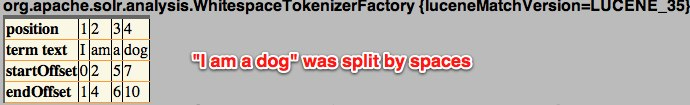
\includegraphics[width=\textwidth]{images/whitespacetokenizerfactory.jpg}

\paragraph{KeywordTokenizerFactory} Treats the entire field as a single token, regardless of its content.
\begin{minted}[fontsize=\scriptsize,linenos]{xml}
<tokenizer class="solr.KeywordTokenizerFactory"/>
\end{minted}

\paragraph{MappingCharFilterFactory} Maps Special characters to their plain equivalent
\begin{minted}[fontsize=\scriptsize,linenos]{xml}
<charFilter class="solr.MappingCharFilterFactory" mapping="mapping-ISOLatin1Accent.txt"/>
\end{minted}
Example (index time): Me alegro de que tú sonrías – It makes me happy that you smile.
\mbox{} \\
\mbox{} \\
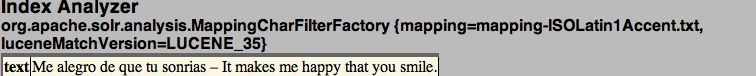
\includegraphics[width=\textwidth]{images/mappingcharfilterfactory.jpg}

\paragraph{LowerCaseFilterFactory} Lowercases the letters in each token. Leaves non-letter tokens alone. 
\begin{minted}[fontsize=\scriptsize,linenos]{xml}
<filter class="solr.LowerCaseFilterFactory"/>
\end{minted}
Example (index time): "I.B.M.", "Solr" ==> "i.b.m.", "solr".
\mbox{} \\
\mbox{} \\
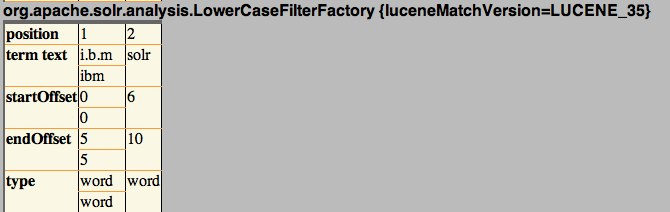
\includegraphics[width=\textwidth]{images/lowercasefilterfactory.jpg}

\paragraph{StopFilterFactory} Discards common words that are listed in the stopwords.txt file. This file is shipped in the module. Examples of these words are "an, and, are, ...". And as visible it comes with some configuration options such as ignoring the case of the text and the file from where to read the stopwords from. This should be a path starting from the conf folder.  When enablePositionIncrements is true a token is stopped (discarded) and the position of the following token is incremented. This is useful if you want to know if certain words were discarded by looking at the token position.
\begin{minted}[fontsize=\scriptsize,linenos]{xml}
<filter class="solr.StopFilterFactory"
    ignoreCase="true"
    words="stopwords.txt"
    enablePositionIncrements="true"/>
\end{minted}
\inputminted[fontsize=\scriptsize,linenos]{xml}{./code_examples/stopwords.txt}
\captionof{listing}{Example of the stopwords file \label{code:stopwordsdefinition}}
Example (index time): Si Hola estoy nick a on
\mbox{} \\
\mbox{} \\
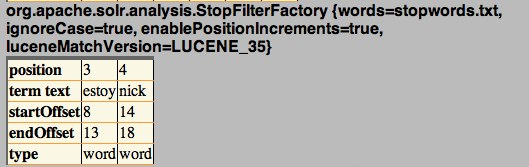
\includegraphics[width=\textwidth]{images/stopfilterfactory.jpg}

\paragraph{WordDelimiterFilterFactory} Delimits words based on parts of words. Was originally defined for the use in english based texts. It follows the following strict order but allows a number of configurations to happen. The original filter has more options but below are only the ones used in the Apache Solr schema.xml
\begin{itemize}
\item{protected} (optional) The pathname of a file that contains a list of protected words that should be passed though without splitting. In the case of Drupal these are predefined as some html entities.
\item{generateWordParts} splits words at delimiters. 
\item{generateNumberParts}  splits numeric strings at delimiters
\item{catenateWords} maximal runs of word parts will be joined: "hot-spot-sensor's" -> "hotspotsensor"
\item{catenateNumbers} maximal runs of number parts will be joined: 1947-32" -> "194732"
\item{catenateAll} Set at 0, runs of word and number parts will not be joined: "Zap-Master-9000" -> "Zap Master 9000"
\item{splitOnCaseChange} words are not split on camel-case changes:"BugBlaster-XL" -> "BugBlaster", "XL"
\item{preserveOriginal} the original token is preserved: "Zap-Master-9000" -> "Zap-Master-9000", "Zap", "Master", "9000"
\end{itemize}
\begin{minted}[fontsize=\scriptsize,linenos]{xml}
<filter class="solr.WordDelimiterFilterFactory"
    protected="protwords.txt"
    generateWordParts="1"
    generateNumberParts="1"
    catenateWords="1"
    catenateNumbers="1"
    catenateAll="0"
    splitOnCaseChange="1"
    preserveOriginal="1"/>
\end{minted}
Example text (index time): Zap-Master-9000 9000-12 BugBlaster-XL hot-spot-sensor's
\mbox{} \\
\mbox{} \\
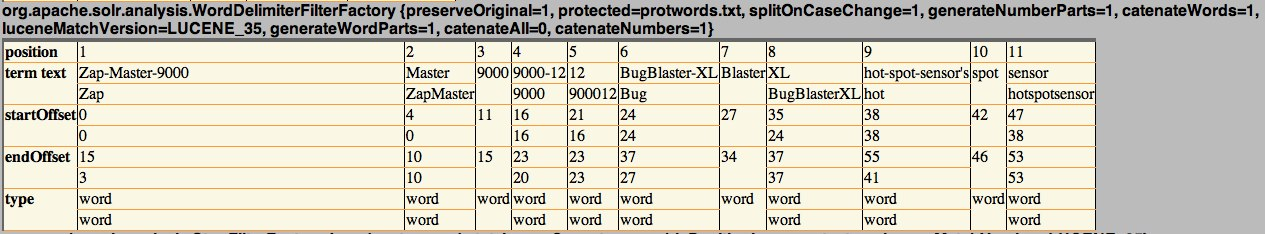
\includegraphics[width=\textwidth]{images/worddelimiterfactory.jpg}

\paragraph{LengthFilterFactory} Words smaller than 2 chars and bigger than 100 will be discarded. This is useful to speed up the query process because a blog posting from large scale solr mentions that a query will be exponentially grow in query time when small  words are used (Add reference!!!)
\begin{minted}[fontsize=\scriptsize,linenos]{xml}
<filter class="solr.LengthFilterFactory" min="2" max="100" />
\end{minted}
Example Text (index time): I am a dog a b c 123
 \seqsplit{iamawordoveronehundredcharactersiamawordoveronehundredcharactersiamawordoveronehundredcharactersiamawordoveronehundredcharactersiamawordoveronehundredcharactersiamawordoveronehundredcharacters}
\mbox{} \\
\mbox{} \\
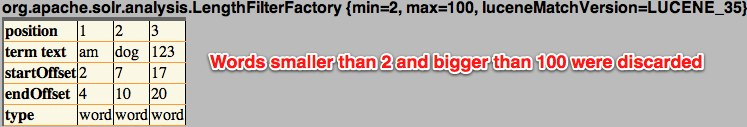
\includegraphics[width=\textwidth]{images/lengthfilterfactory.jpg}

\paragraph{SynonymFilterFactory} This is quite a special one that is only executed during query time. Meaning that words will not be processed as synonyms in index time. If a user would type color it could also check the index for texts with the word "colour". Same is valid for the more concrete example "GB,gib,gigabyte,gigabytes"
\begin{minted}[fontsize=\scriptsize,linenos]{xml}
<filter class="solr.SynonymFilterFactory" synonyms="synonyms.txt" ignoreCase="true" expand="true"/>
\end{minted}
Example Text (query time): colour test
\mbox{} \\
\mbox{} \\
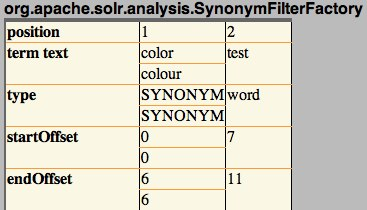
\includegraphics[width=\textwidth/2]{images/synonymfilterfactory.jpg}

\paragraph{TrimFilterFactory} This filter trims leading and/or trailing whitespace from tokens. In Drupal usecase this is used for sortable text such as names or labels. The big difference with most other filters is that this filter does not break words on spaces.
\begin{minted}[fontsize=\scriptsize,linenos]{xml}
<filter class="solr.TrimFilterFactory" />
\end{minted}
Example Text (query time): Nick Veenhof
\mbox{} \\
\mbox{} \\
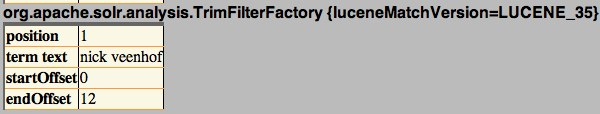
\includegraphics[width=\textwidth]{images/trimfilterfactory.jpg}

\paragraph{EdgeNGramFilterFactory} This filter generates edge n-gram tokens of sizes within the given range. In the module it was configured to return 2-gram tokens till 25-gram tokens. Especially useful for matching against queries with results. \footnote{\url{http://www.lucidimagination.com/blog/2009/09/08/auto-suggest-from-popular-queries-using-edgengrams/}}
\begin{minted}[fontsize=\scriptsize,linenos]{xml}
<filter class="solr.EdgeNGramFilterFactory" minGramSize="2" maxGramSize="25" />
\end{minted}
Example Text (index time) : I am a dog with a longbigtext
\mbox{} \\
\mbox{} \\
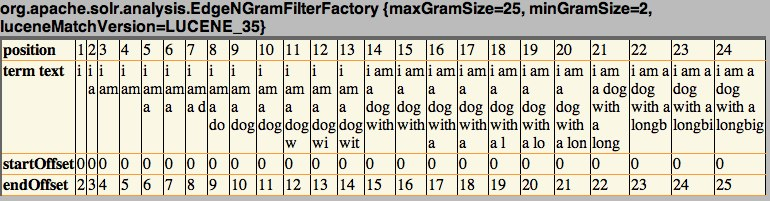
\includegraphics[width=\textwidth]{images/edgengramfilterfactory.jpg}

\paragraph{SnowballPorterFilterFactory} Snowball is a software package that generates pattern-based word stemmers. It works efficiently and fast and one can configure the language that is preferred. Apache Solr comes with a whole range of languages. English is very well supported but also Catalan and Spanish. A list of all the languages can be found in the documentation of Apache Solr or in the Snowball website \footnote{\url{http://snowball.tartarus.org/}}. Also interesting to note is that there is a file called protwords.txt (Protected words) where you can define strings that won't be stemmed.
\begin{minted}[fontsize=\scriptsize,linenos]{xml}
<filter class="solr.SnowballPorterFilterFactory" language="English" protected="protwords.txt"/>
\end{minted}
Example Text (index time) : football footballing
\mbox{} \\
\mbox{} \\
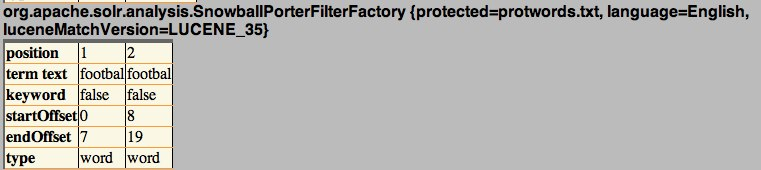
\includegraphics[width=\textwidth]{images/snowballporterfilterfactory.jpg}

\paragraph{RemoveDuplicatesTokenFilterFactory} Removes duplicates from the query or the index value.
\begin{minted}[fontsize=\scriptsize,linenos]{xml}
<filter class="solr.RemoveDuplicatesTokenFilterFactory"/>
\end{minted}
Example : Nick Nick Nick

\paragraph{Speed} Speed is an important factor. During the research phase I found an interesting article \footnote{\url{http://www.hathitrust.org/blogs/large-scale-search/slow-queries-and-common-words-part-1}} that showed a graph of the response time for their index. 
This graph shows that 97\% of the requests were completed in less than a second. The average was found to be 673 milliseconds. Those 3\% of the queries are slower because there is a longer disk seek time. This means that some queries contains commonly occurring words such as "a", "of", "the", "and", etc... Queries with common words take longer because the data structures containing the lists of documents containing those words in the index are larger.
This same source mentions that the common\-grams filter \footnote{\url{http://wiki.apache.org/solr/AnalyzersTokenizersTokenFilters\#solr.CommonGramsFilterFactory}} for Apache Solr could resolve these queries but further investigation is due. As a conclusion it can be said that Apache Solr is a very fast add-on to Apache Lucene for full text searching, spelling corrections, faceted search and much more.

\begin{figure}[H]
     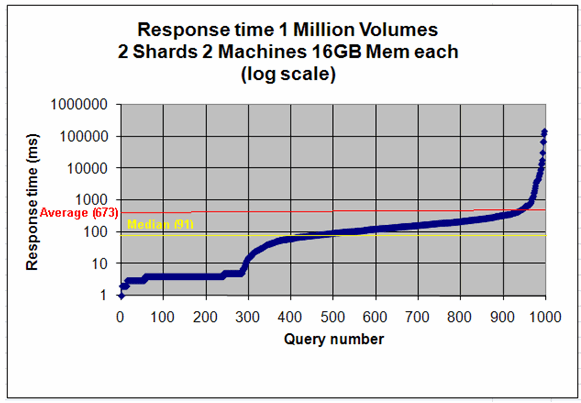
\includegraphics[width=\textwidth]{images/response_time.png}
     \caption{Response Time for a Solr Index with over 1 Million records (Logarithmic Scale)}
\end{figure}


\paragraph{Dynamic Fields in Solr used by Drupal}
As explained, using a combination of Field types and field properties a schema can create lots of dynamic configurations for softwares that interact with Solr. In the case of Drupal the ApacheSolr Drupal module does not know in advance how the schema should look like because all Drupal sites are differently configured using different content types. The module should be able to cope with most of the use cases that site administrators come up with. If a field name is not found while submitting a new document, dynamicFields will be used if the name matches any of the patterns. Note that there are restrictions namely that the glob-like pattern in the name attribute must have a "*" only at the start of the end of the field definition. For example, name="\*\_i" will match any field ending in \_i (like myid\_i, z\_i). Longer patterns will be matched first and if equal size patterns both match, the first appearing in the schema will be used.
 
Before starting this work not all of these dynamic fields were provided to the site administrators but with time a list was compiled to meet 99\% of the use cases.  See schema.xml in the project files for the complete list. A small snippet of some of these dynamic fields is included below. The 1st letter indicates the data type and the last letter is 's' for single valued, 'm' for multi-valued.

\inputminted[fontsize=\scriptsize,linenos]{xml}{./code_examples/schema_dynamicfields.xml}
\captionof{listing}{Example of some dynamic field type definitions \label{code:fielddynamicdefinition}}

\noindent In the implementation chapter it will be explained how these dynamic fields are used to create new fields in solr using Drupal.


\section{Standard Drupal Search}
By default Drupal already ships with a search module that leverages Mysql to its far extent in order to create a search experience that works quite well in smaller scale websites.

In Drupal there is a concept called "cron". These are actions that are executed per a set amount of time, for example 30 minutes. Every 30 minutes the designated search actions will index a little set of the selected content, for example 100 pages. This will run until there is no more content to index. Naturally content will change and will need to be re-indexed. This concept is fairly basic and is also the one used for the Apache Solr module. 
However, I'd like to point out that the Search module that is shipped with Drupal differs greatly from the Apache Solr module. 

\paragraph{Advantages} The standard Drupal search module certainly has its advantages. There is, to start with, no extra server/service necessary and it does ship with Drupal core. The basic module also has support for basic text transformations, such as recognition of singular and plural words. It transforms special characters to basic text characters (Similar to the MappingCharFilterFactory in Apache Solr) and it scores items based on their tag where they are embedded in. Examples are H1, H2 and P tags.

\paragraph{Disadvantages} However, it has a hard time handling a big data set. MySQL was not built to be a search engine. Mysql also has its limitations when building a full text search on top of its stack. Drupal also has to comply with the SQL standards so engine specific optimizations cannot be utilized. \footnote{\url{http://dev.mysql.com/doc/refman/4.1/en/fulltext-restrictions.html}}. This leaves the SQL solution with a very restricted set of operators and inherently slow and not scalable in the long haul. 

\paragraph{Conclusion Drupal SQL search} An SQL backend does well in serving a full text search application as long as the number of indexed items stay stable and preferably < 10000 items. \footnote{This number is an estimation, depending on the SQL database application and server configuration this can vary greatly}

\section{Apachesolr Search Integration Drupal Module}
The module found its origin around the end of 2007, at the time of Drupal 5. It's first author was Robert Douglass and lots of other people followed his lead in this initiative. Fast forward and at the moment of writing a Drupal 6 and 7 version exist. When this work started the Drupal 7 version was basically a port of the Drupal 6 version and needed lots of improvements. Acquia sponsors development of this module to ensure continuity and support.

\paragraph{Filtering}
Search facets, also known as filters allow users to refine or sort their search result set. Users can begin with a general search and narrow down the result set as they understand better what content is available on a site.

\begin{wrapfigure}{l}{0.3\textwidth}
\begin{center}
     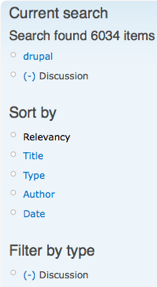
\includegraphics[width=0.25\textwidth]{images/Search_facet_ex_4_by-type-ex-1.png}
     \caption{Filter by Type example. A user clicked on Discussion}\end{center}
\end{wrapfigure}
\paragraph{}
When a user clicks on any term within a filter block it sends a new query to the Apache Solr server and it returns a resultset with the narrowed down results so it only includes content that matches the original query (text search) and the newly selected filter. 
The practice of this narrow-down method is that the user can keep selecting new filters until he found what he was looking for. The facets can be configured as OR or AND. When the user clicks the minus "(-)" the filter will be removed from the current set and show the results of the search minus that specific filter.

\begin{wrapfigure}{r}{0.60\textwidth}
\begin{center}
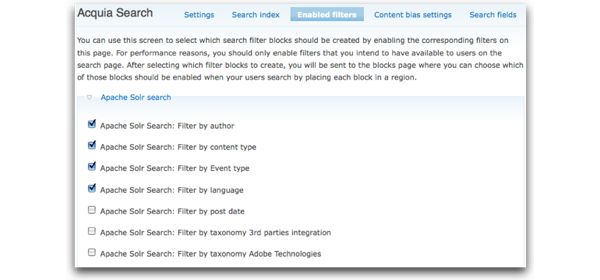
\includegraphics[width=0.60\textwidth]{images/enabled_search_filters_page-1.png}
\caption{Configure the facets}
\end{center}
\end{wrapfigure}

\paragraph{Configuration} When the site creator wants to add more facets it is possible by going to a configuration page. as shown in the picture above. The site creator selects the facets he wants and then configures them in more detail in the block settings. The block configuration page allows you to configure, for example, the number of filters the block displays, how many it displays after clicking the show more link, the title of the block and many more. Some important facets to mention are Author, Content Type, Language, Vocabulary and Dynamic CCK/Field API filters

\paragraph{Content Recommendation}
Apache Solr can also show content suggestions to user that is viewing a specific piece of content. These suggestions are made based on the content of the viewed text. It can be used for suggestions similar to "customers who bought X also liked Y", or simply a list of relevant blog entries. The importance of certain parameters can be adjusted in the bias settings.
\begin{figure}[H]
     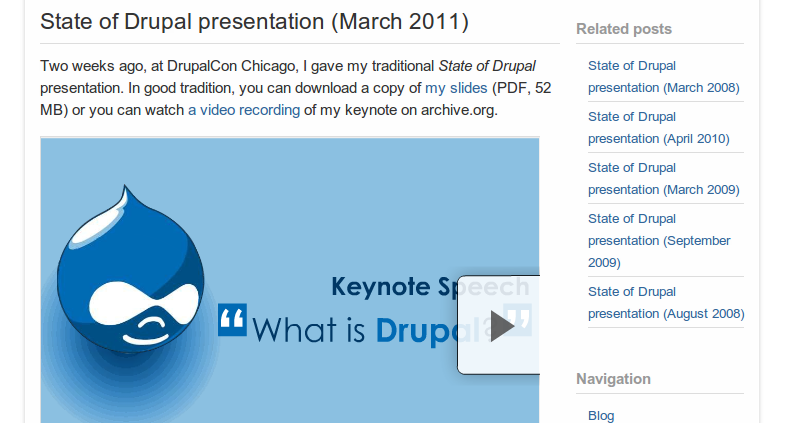
\includegraphics[width=\textwidth]{images/more_like_this.png}
     \caption{Content Recommendations can be seen in the block "Related Posts"}
\end{figure}

\begin{wrapfigure}{l}{0.5\textwidth}
\begin{center}
     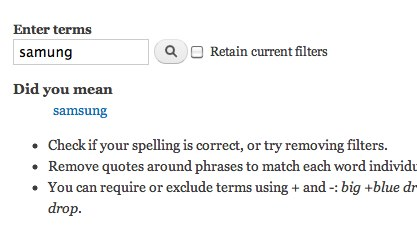
\includegraphics[width=0.5\textwidth]{images/spellchecker.jpg}
     \caption{Spelling correction}
\end{center}
\end{wrapfigure}
\paragraph{Spelling Suggestions}
One of the other features of Apache Solr, and a feature that conquered a lot of hearts in the community was the spellchecker. Similarly to what Google does when you misspell a word it will search in the index for a word similar to your word, but with better/more relevant results.

\paragraph{State of the UI as of September 2011} What is shown below is a snapshot of how the module looked in the backend as of September 2011. There are markers that indicate problem area. Do take into account that this does not show you any comments made on the internals of the module.
\begin{figure}[H]
     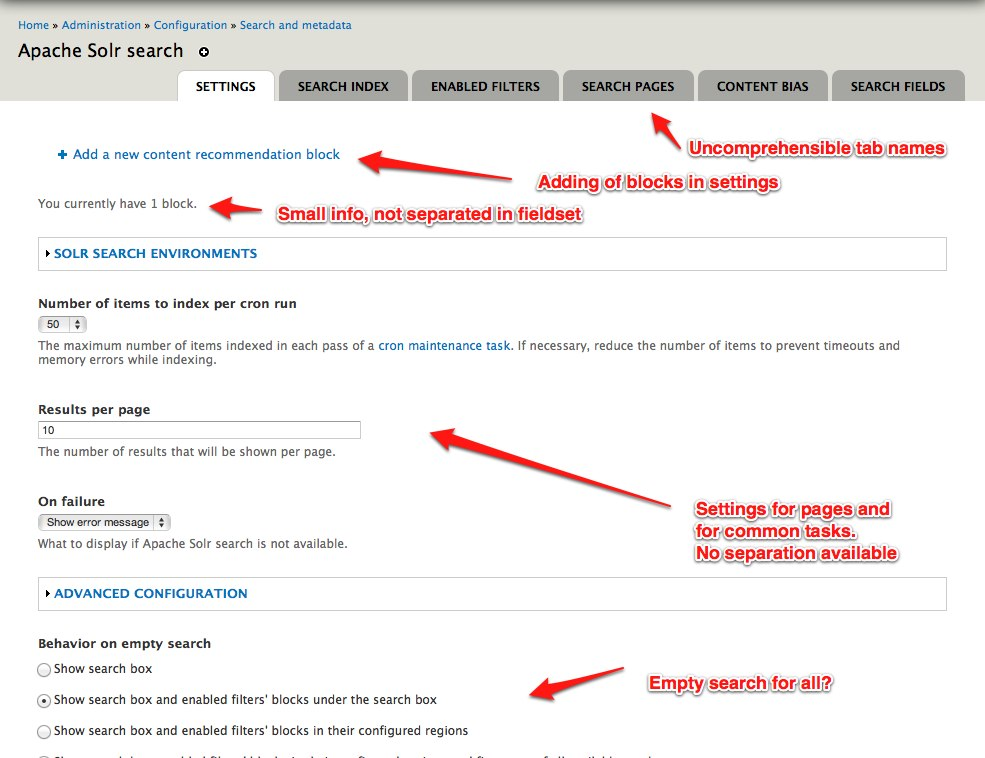
\includegraphics[width=\textwidth]{images/apachesolr_ui_backend_september_2011_1.jpg}
     \caption{UI settings backend, September 2011}
\end{figure}
\paragraph{Summary for the UI settings backend}
\begin{itemize}
\item The tab names are hard to understand. Search bias and/or Search fields are not comprehensible for a first time user.
\item The first like is a link to add a content recommendation block. Surely there must be more important items to appear at the top. 
\item In the settings tab there are global search page settings and ideally those must be generalized so that each search page can use another preset.
\item The use of the "Show search box" appears everywhere and is therefor obsolete.
\end{itemize}

\begin{figure}[H]
     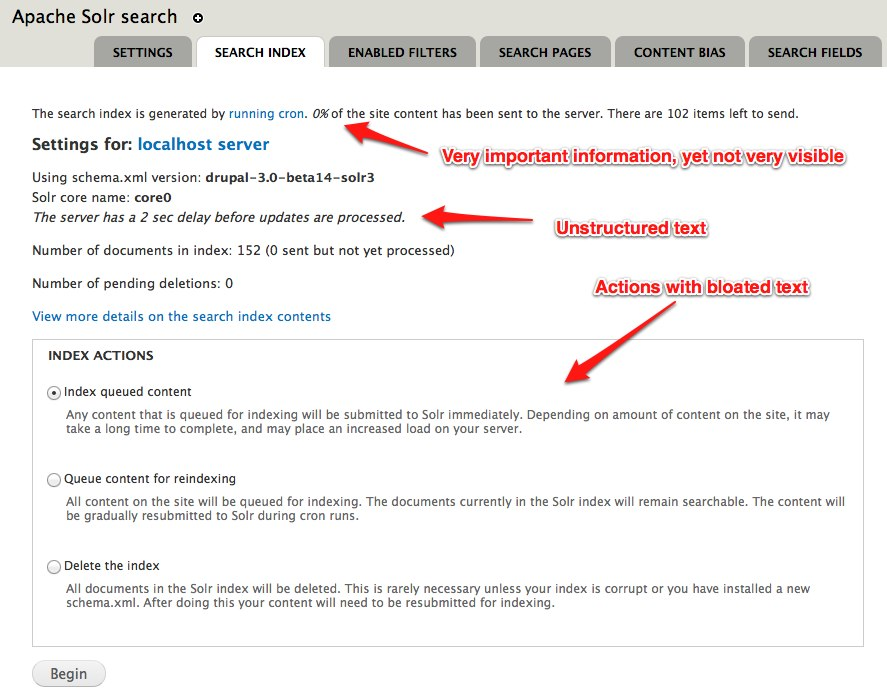
\includegraphics[width=\textwidth]{images/apachesolr_ui_backend_september_2011_2.jpg}
     \caption{UI index report backend, September 2011}
\end{figure}
\paragraph{Summary for the UI report backend}
\begin{itemize}
\item There is information spread out across the whole page. This should be structured and weight should be given to the more important parts.
\item There are 3 types of actions but reading all of them makes you doubt even more about what they do. That should be clarified
\end{itemize}


\begin{figure}[H]
     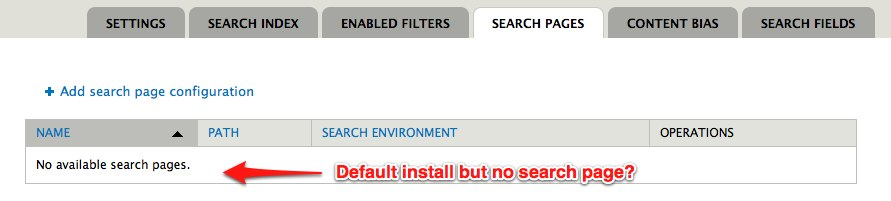
\includegraphics[width=\textwidth]{images/apachesolr_ui_backend_september_2011_3.jpg}
     \caption{UI search pages backend, September 2011}
\end{figure}
\paragraph{Summary for the UI search pages backend}
\begin{itemize}
\item When going to the search pages the first time, the user sees that the list is empty. However, when going to the search in Drupal a new search tab was added. This raises confusion and therefore the core search page (overtaken by Apache Solr) should appear in the search pages listing.
\end{itemize}

\begin{figure}[H]
     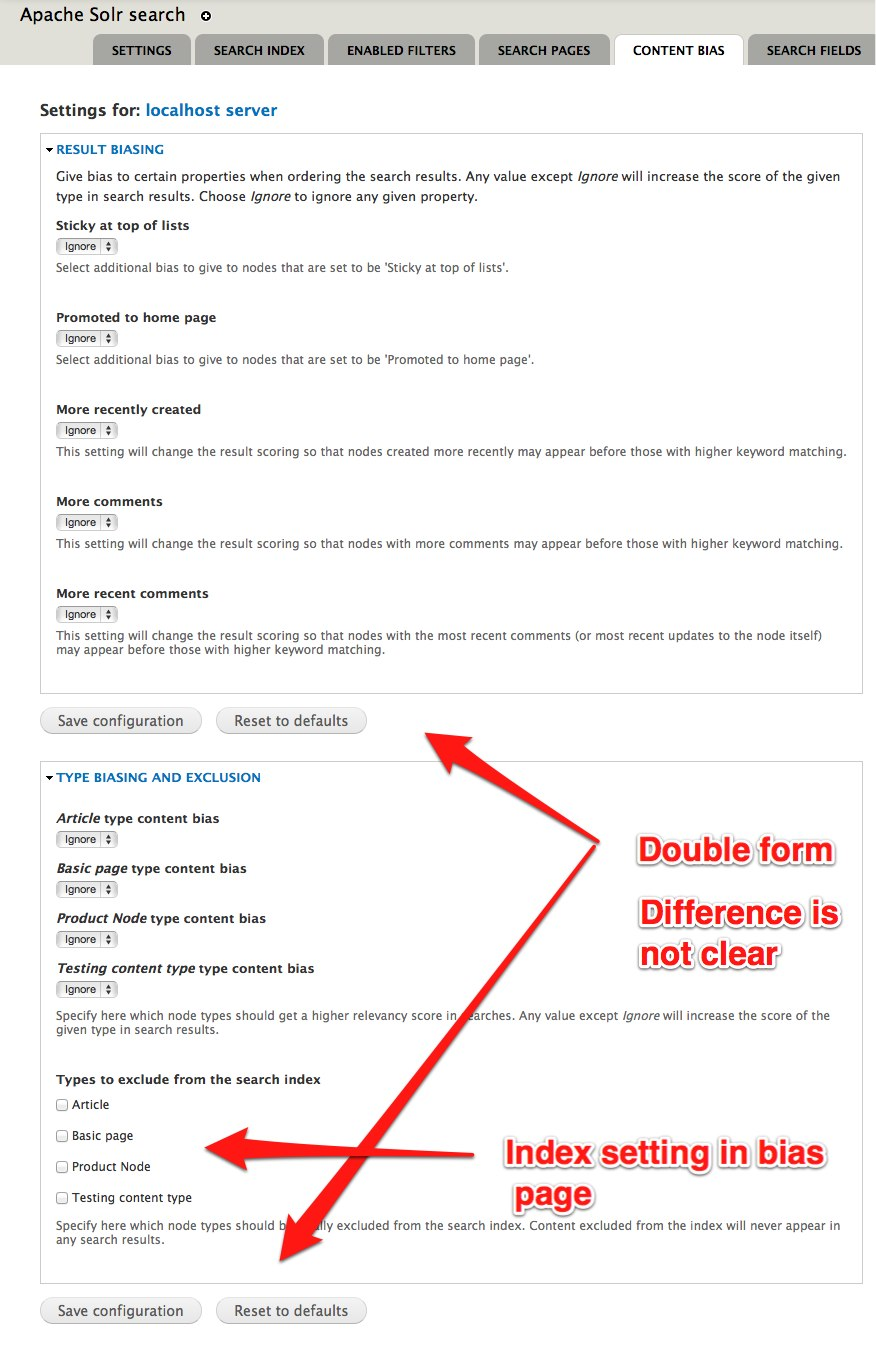
\includegraphics[width=\textwidth/(2)]{images/apachesolr_ui_backend_september_2011_4.jpg}
     \caption{UI for result and index biasing backend, September 2011}
\end{figure}
\paragraph{Summary for the UI index biasing backend}
\begin{itemize}
\item Multiple forms are visible in 1 page. According to the UI standards of Drupal this is a no-go.
\item it also appears there is a settings available, a setting that excludes content types from the index, that should be moved to the index settings. 
\end{itemize}

\paragraph{Architectural challenges}
Drupal and the module were never intended to be built by architects but by people who solve problems, real world problems. Many people worked together to create a cohesive project that is very stable but might not be in agreement with that is taught in classes such as Object Oriented programming, other theories and best practices. A class diagram would be a faulty way to show you the beauty this module has to offer its users since there were hardly object oriented concepts applied to this module that were worthy enough to show a class diagram from. Together with Acquia we've set up a list of minimal achievements that should be reached by the end of  February. Some of these items are also issues that were pointed out by other companies or users and they were being put into the issue queue waiting for an answer or a resolution. 

\paragraph{Improvements}
\begin{packed_itemize}
\item UI refactoring to make a better experience \footnote{\url{http://drupal.org/node/1292364}}
\item Support the indexing of multiple entities natively so the module would have an API to index users / terms / ... easily \footnote{\url{http://drupal.org/node/1292364}}
\item Global functions should be context driven.\footnote{\url{http://drupal.org/node/1292364}}
\item Get rid of dependencies in theme layer from core search \footnote{Related to \url{http://drupal.org/node/1314406} (de-duplication)}
\item (Performance) Hooks node\_type, taxonomy and user knocks out our database server \footnote{\url{http://drupal.org/node/592522}}
\item Improve file listing and access control
\item More like this blocks should get a delete button \footnote{\url{http://drupal.org/node/1271964}}
\item De-duplicate core and custom search in order to obtain clarity in the code \footnote{\url{http://drupal.org/node/1314406}}
\item Add 1 custom search block with generic render function for custom development
\item The numeric field id should not be used for Solr index field names \footnote{\url{http://drupal.org/node/1161538}}
\item Query type should be adjusted in order to allow different widgets in facetapi \footnote{\url{http://drupal.org/node/1161444}}
\item Change the PHP static to the Drupal function drupal\_static() \footnote{\url{http://drupal.org/node/1334216}}
\item Non-current/valid Node Types are not excluded from index \footnote{\url{http://drupal.org/node/1000532}}
\item Add retain current filters checkbox to custom search page \footnote{\url{http://drupal.org/node/1246422}}
\item Add "retain-filters" param when in facet browsing mode \footnote{\url{http://drupal.org/node/1116792}}
\item Handle 1 placeholder in a custom search page path with makes the taxonomy sub-module obsolete \footnote{\url{http://drupal.org/node/1294846}}
\item Create tests for the module \footnote{\url{http://drupal.org/node/989398}}
\item Bundle' is not a required field, but Apachesolr treats it as such (Evaluate required fields in schema, make non-required if possible) \footnote{\url{http://drupal.org/node/1279164}}
\item Improve Date faceting/date query type (combined with facetapi) \footnote{\url{http://drupal.org/node/1201534}}
\item Facets are currently not linked to the appropriate search page
\item Add clone operation for search environments \footnote{\url{http://drupal.org/node/1292328}}
\item Backport Apache Solr Module to Drupal 6
\end{packed_itemize}

\section{Facetapi Drupal module}
The Facet API module allows site builders to easily create and manage faceted search interfaces. In addition to the UI components that come out of the box, themers and module developers can build their own widgets that can optionally be contributed back to Drupal.org. Facet API works with the core Search, Search API, and Apache Solr Search Integration modules (including Acquia Search) meaning that code and configuration can be reused as-is with the most popular search solutions available to Drupal. It was created by Chris Pliakas and Peter Wolanin specifically for the Drupal 7 version of any search tool. Acquia sponsors development of this module to ensure continuity and support.

\paragraph{State of the UI as of September 2011} What is shown below is a snapshot of how the module looked in the backend and frontend as of September 2011. There are markers that indicate problem area. Do take into account that this does not show you any comments made on the internals of the module.

Screenshots of the implemented part of facetapi (Drupal 7)
\begin{figure}[H]
     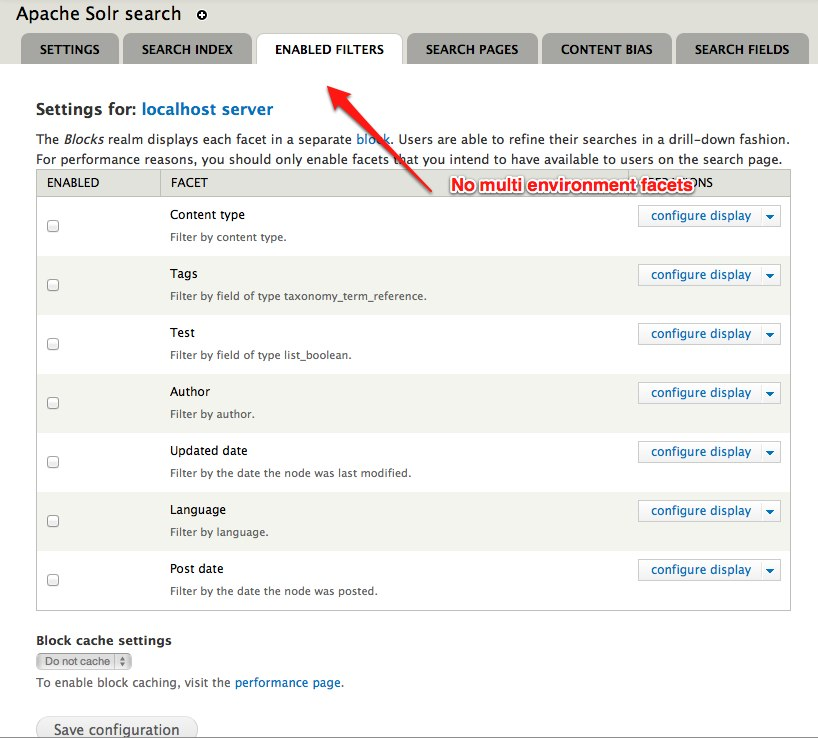
\includegraphics[width=\textwidth]{images/facetapI_ui_september_2011.jpg}
     \caption{Apachesolr Facetapi Integration UI as of September 2011}
\end{figure}
\paragraph{Summary for the UI search pages backend}
\begin{itemize}
\item There was no possibility to easily switch to facets from other environments because one had to make the other environment the default one. This was a huge workaround and had to be fixed.
\end{itemize}

\begin{figure}[H]
     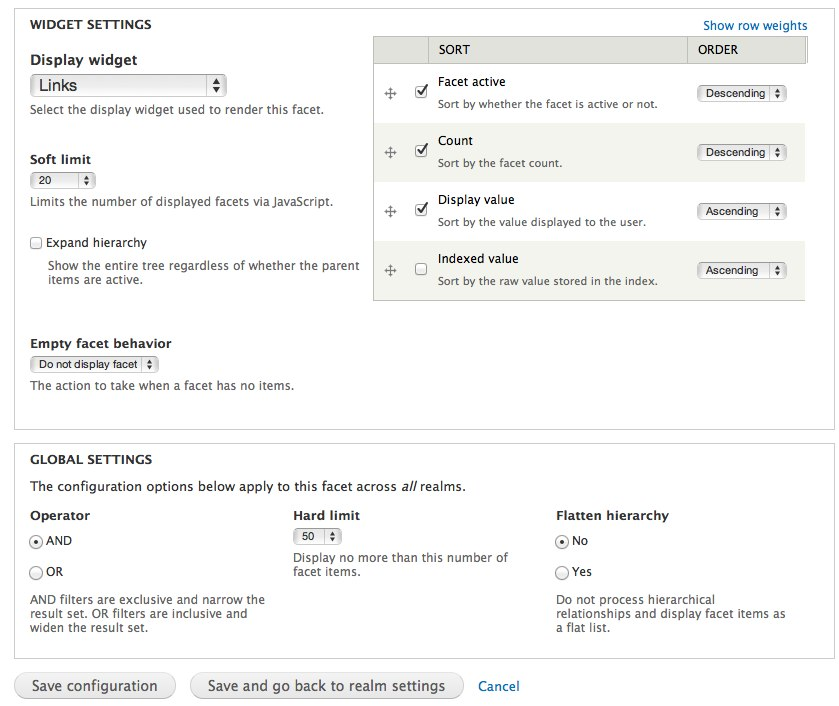
\includegraphics[width=\textwidth]{images/facetapi_ui_facet_september_2011.jpg}
     \caption{Apachesolr Facetapi Integration UI of 1 facet as of September 2011}
\end{figure}
\begin{itemize}
\item The Facet details page was ok in its use and therefor it did not need any further adjustments.
\end{itemize}

\paragraph{Architecture}
As part of the analysis a class diagram was made from the Facet Api code to get a better understanding of the internals. An issue \footnote{\url{http://drupal.org/node/1321136}}was raised in the Facet Api issue queue on \url{drupal.org} for those that prefer to read up in detail.

\begin{figure}[H]
     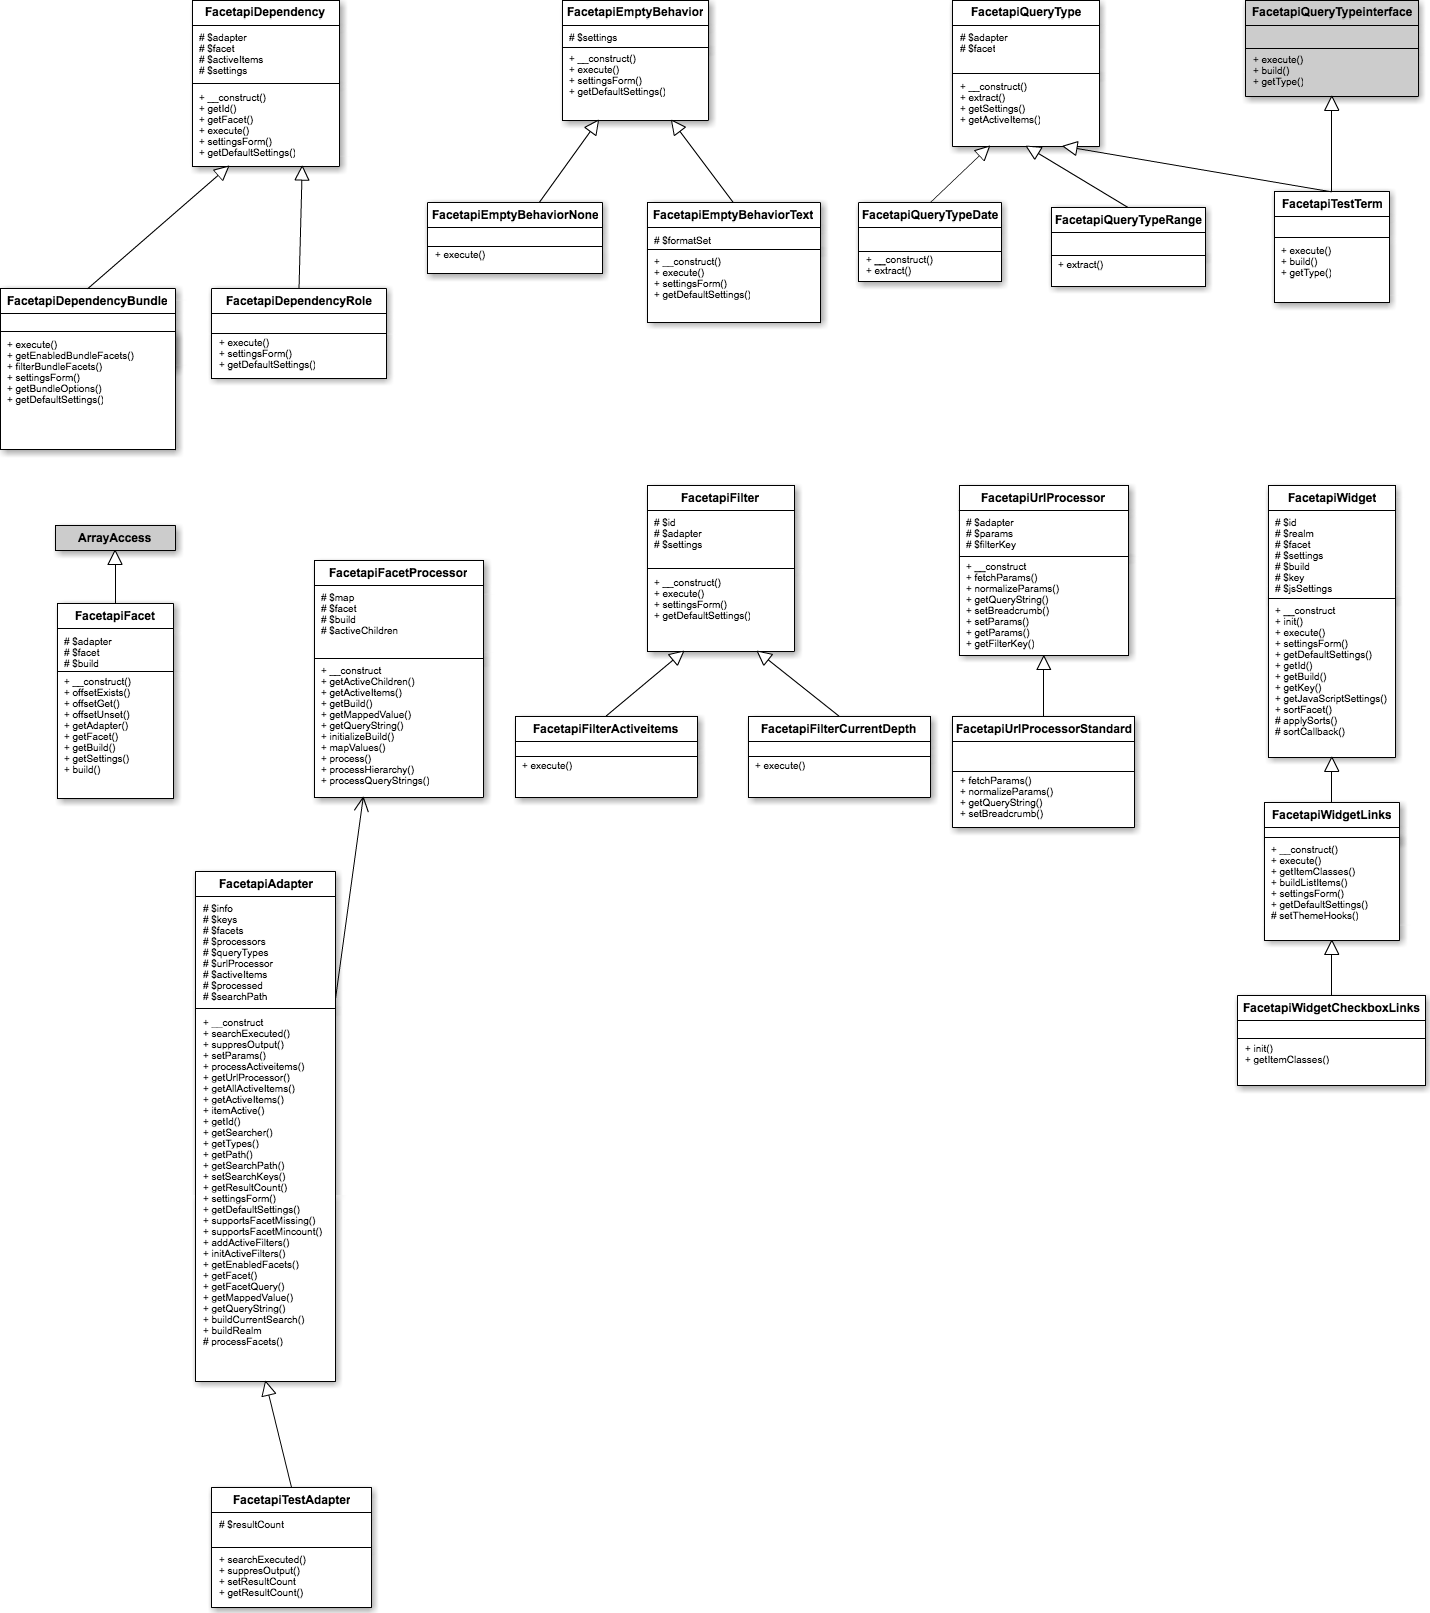
\includegraphics[width=\textwidth]{images/facetapi_classdiagram.png}
     \caption{Extended information about the classes in FacetAPI, September 2011}
\end{figure}

\begin{figure}[H]
     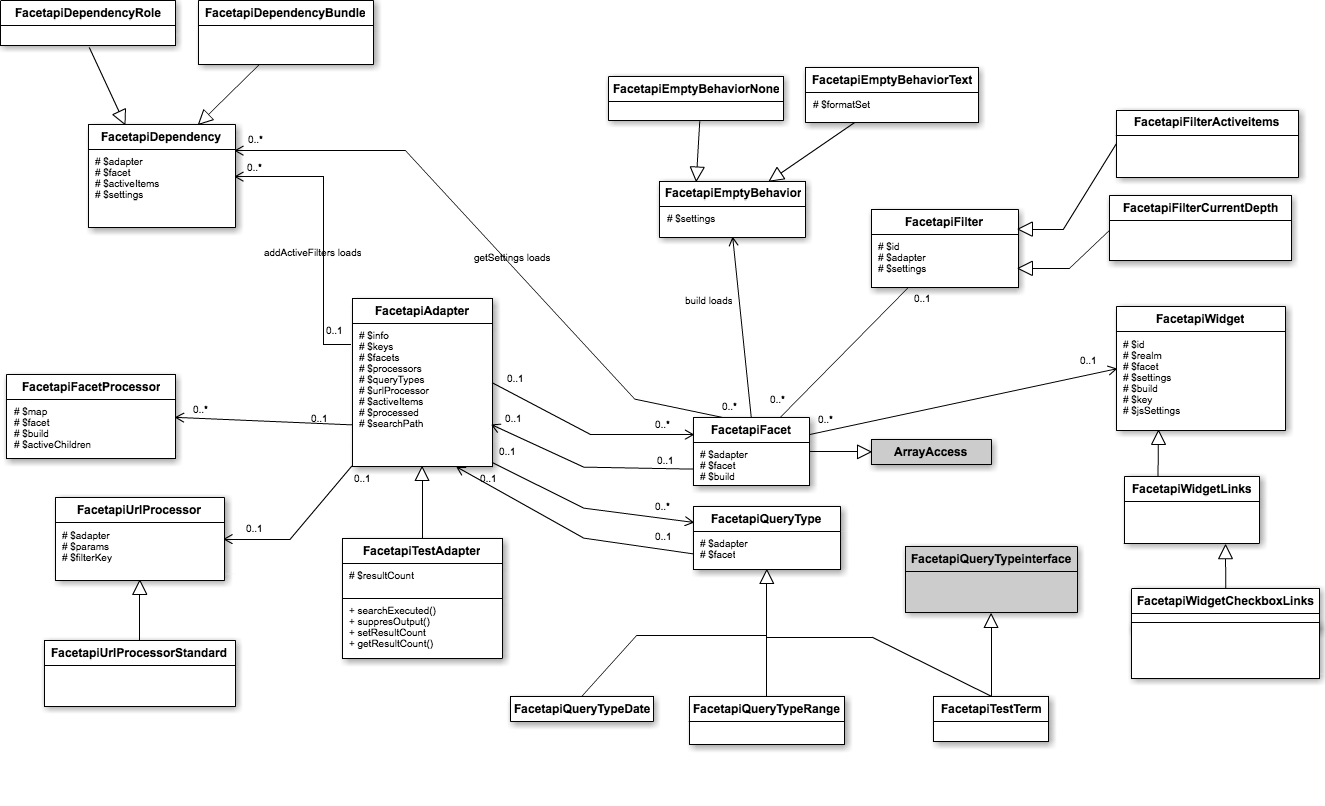
\includegraphics[width=\textwidth]{images/ClassDiagram_facetapi.png}
     \caption{Class Diagram of FacetAPI, September 2011}
\end{figure}

\begin{itemize}
\item There are a number of loop-references between the adapter and it's relations. This can possibly be avoided by thinking the architecture through (see the references that have 2 lines to each other)
\item The variable facet in FacetapiFacet might be a bit too un-descriptive and it looks like it could be renamed to "settings" or "facet\_settings"
\item Doxygen documentation with loads of diagrams and easy to read documentation was generated from this. In addition to the attached images it should make the facetapi module easier to understand. The documentation can be found on \url{http://facetapi.nickveenhof.be}
\end{itemize}

\paragraph{Improvements}
\begin{packed_itemize}
\item Modify "query type" key in facet definition to accept an array \footnote{\url{http://drupal.org/node/1161434}}
\item Make the current search block more configurable \footnote{\url{http://drupal.org/node/593658}}
\item Complete configuration import functionality \footnote{\url{http://drupal.org/node/1147564}}
\item widget.inc change id/class to not reflect the field\_id but a generic one for multisite (line 106) + apachesolr.module line 1860 to remove the id (integer) assumptions
\item Backport Facet Api to Drupal 6
\end{packed_itemize}

\section{Acquia Search for Drupal 6 and 7}
Quote from Dries' blog : "Acquia Search is a hosted search service based on the Software as a Service (SaaS) model. The way it works is that Drupal sites push their content to the search servers hosted by Acquia. We index the content, builds an index, and handle search queries. We provide the search results, facets, and content recommendations to your Drupal site over the network." \footnote{\url{http://buytaert.net/acquia-search-benefits-for-site-administrators}}

As the reader of this paper would have guessed, Acquia Search is built using the Open Source Lucene and Solr distributions from the Apache project. Another quote from Dries' website : "Many organizations simply lack the Java expertise to deploy, manage and scale Java applications or their hosting environment may not accommodate it. Because Acquia Search is a hosted service, it takes away the burden of installation, configuration, and operational duties to keep the software fast, secure and up-to-date."

\paragraph{Architecture}
\begin{figure}[H]
     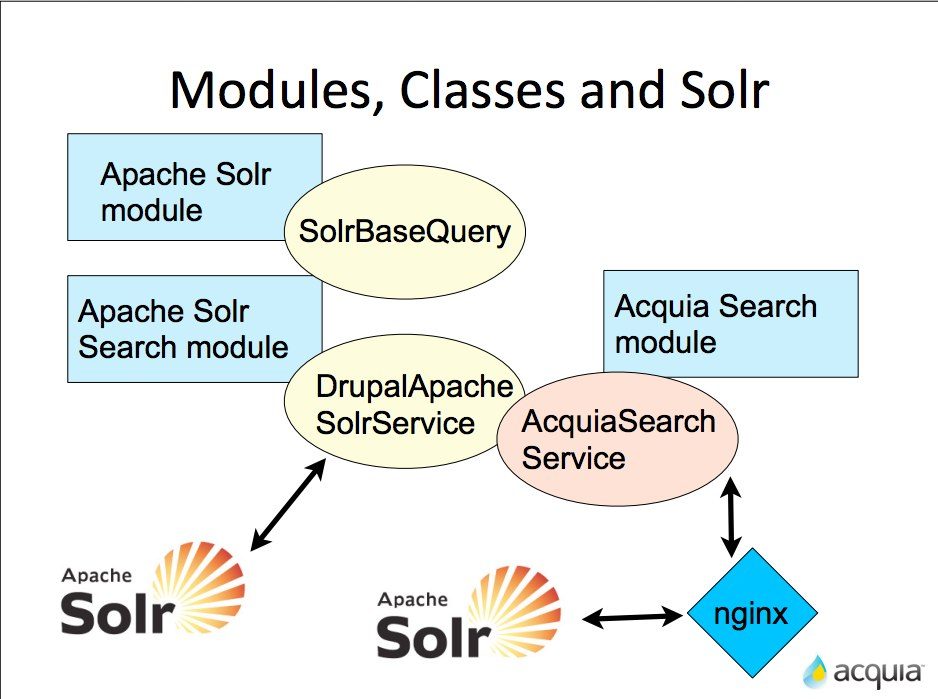
\includegraphics[width=10cm]{images/acquia_solr_classes.jpg}
     \caption{Overview of the classes and services used for Acquia Search at the website's end.}
\end{figure}

Even though the image was not build as a real class diagram it should be clear that there are 2 classes in the Apache Solr module that are pictured here (yellow). The only important one to cover here is the DrupalApacheSolrService. This class makes it possible to connect to an arbitrary Solr server. When the Acquia Search module is enabled on any website the AcquiaSearchService class extends the DrupalApacheSolrService class and adds the authentication information to all the requests.

The next figure will explain the server side handling of the requests that are being sent to Solr.
\begin{figure}[H]
     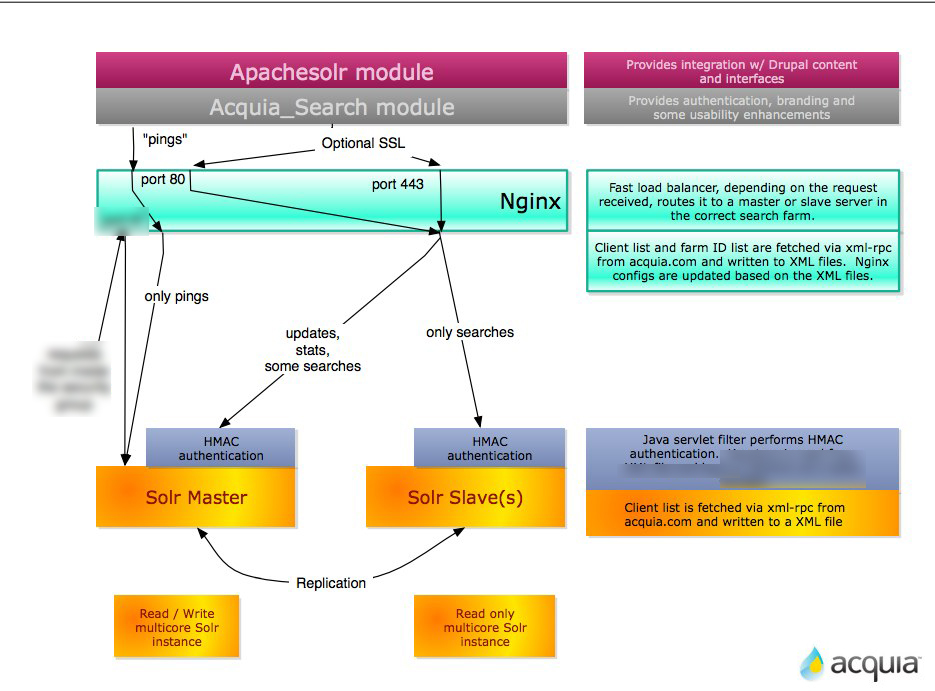
\includegraphics[width=\textwidth]{images/acquia_architecture.jpg}
     \caption{Server Side view of Acquia Search. Certain information has been blurred for confidentiality}
\end{figure}

\paragraph{HMAC authentication filter}
The way it works is that the data is protected during the transport over the web by SSL and to authenticate to the search servers at Acquia an SHA1-HMAC authentication layer is used. This means that the data is encrypted so no man in the middle attack can be exploited. Acquia knows that you have sent the request and will verify, using this SHA1-HMAC authentication, if the data that was sent was not modified. 

This kind of authentication is commonly called a symmetric signature. Using a shared secret the message is signed and also verified as can be seen in the image below.

\begin{figure}[H]
     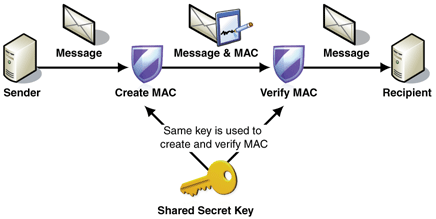
\includegraphics[width=10cm]{images/IC42720.png}
     \caption{Signing a message using a symmetric signature}
\end{figure}

As illustrated in the figure above, signing a message using a symmetric signature involves the following steps:

\begin{itemize}
\item The sender creates a HMAC using a shared secret key and attaches it to the message.
\item The sender sends the message and HMAC to the recipient.
\item The recipient verifies that the HMAC that was sent with the message by using the same shared secret key that was used to create the HMAC.
\end{itemize}

By signing with a shared secret, both data integrity and data origin authenticity are provided for the signed message content. The only downside is that the receiver does not know who exactly wrote the message. It can only verify if it was encrypted with the right shared key. Acquia Search creates a hash from the network identifier (aka the subscription ID from the customer) and generates a secret shared key from this information. Using this derived key and a blob of data it can be easily encoded so the backend is able to verify the authenticity of the message

\inputminted[fontsize=\scriptsize,linenos]{php}{./code_examples/hmac_snippet.php}
\caption{Small excerpt to show how the Client side generates the HMAC message to send back to the Solr Service}

\paragraph{State of Acquia Search}
When the internship started at Acquia there were some blanks left to be filled regarding Acquia Search. Since Solr 3.4 (now 3.5) came out it was only a logical step to convert the Acquia Search service to this newer version of Apache Solr so it could be used in the software as a service ideology that Acquia has. The version that is currently used is Apache Solr 1.4 and is still one of the defacto standards when deploying Solr.

As always,  upgrading does not usually happen overnight without any effort. There are many clients running their active sites from Solr 1.4 and it is not guaranteed that all of these will work perfectly for Solr 3.5. Performance factors are also a key role during this migration. 

As reviewed by the architecture it also needs a confirmed upgrade path for the HMAC authentication, which was written specifically for Solr 1.4 as a Java Servlet.

\paragraph{Improvements}
\begin{itemize}
\item Upgrade the Java Servlet that was written to handle HMAC authentication Solr request to Solr 3.x
\item Test if the Solr 3.x performs better or equally good using the upgraded code and by using existing indexes and a real infrastructure server setup to emulate a real-life situation.
\end{itemize}